
\subsubsection{16.10.14}

\begin{enumerate}
	\item Время начала и окончания собрания:
	17:00 - 21:00
	\item Цели собрания:
	\begin{enumerate}
	  \item Подключить контроллер для сервоприводов и подсоединить к нему сервопривод захвата.
	  
	  \item Включить в программу управления роботом управление захватом.
	  
	  \item Доработать подъемник.
	  
    \end{enumerate}
	\item Проделанная работа:
	\begin{enumerate}
	  \item К сегодняшнему занятию мы приобрели алюминиевую полосу 100 см х 4 см х 0,3 см для создания поперечных балок для попарного скрепления направляющих (далее они будут называться ребрами жесткости) и алюминиевую ось длиной 100 см и диаметром 8 мм для создания перекладин.
      
      \item  Полоса была распилена на 4 сегмента нужной длины. Для того чтобы установить получившиеся поперечные ребра жесткости на робота, было решено приобрести Г-образный профиль и распилить его на уголки нужного размера.
      
      \item  Метровой оси хватило на 4 перекладины из необходимых 6. Две из них были закреплены с помощью деталей из набора TETRIX. Для еще одной были просверлены отверстия, однако она не была жестко закреплена. Последнюю ось, предназначенную для самой внутренней пары направляющих, было решено пока не устанавливать: во-первых, мы пока не придумали, как это сделать, а во-вторых это бы осложнило доработку подъемника.
      
      \item   Нами был установлен контроллер сервоприводов и к нему был подключен сервопривод свободного вращения, отвечающий за захват мячей.
      
      \begin{figure}[H]
      	\begin{minipage}[h]{1\linewidth}
      		\center {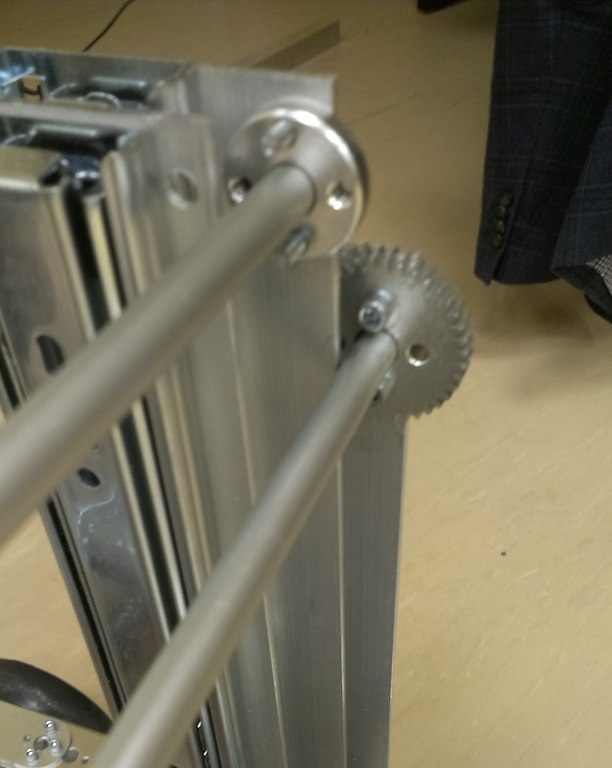
\includegraphics[scale=0.25]{days/16.10.14/images/01}}
      		\caption{Перекладины, установленные на робота} 
      	\end{minipage}
      	%\hfill
      %	\begin{minipage}[h]{0.5\linewidth}
     % 		\center{
\includegraphics[scale=0.4]{days/16.10.14/images/02}}
      %		\caption{Контроллер сервоприводов}
      %	\end{minipage}
      \end{figure}
      
    \end{enumerate}
    
	\item Итоги собрания: 
	\begin{enumerate}
	  \item Установлен контроллер сервоприводов.
	  
      \item Программа управления сервоприводом не написана.
      
      \item Алюминиевая полоса распилена на ребра жесткости, готовые к закреплению на роботе.
      
      \item Ось распилена на перекладины.
      
    \end{enumerate}
    
	\item Задачи для последующих собраний:
	\begin{enumerate}
	  \item Купить еще одну алюминиевую ось и напилить из нее оставшиеся перекладины.
	  
	  \item Купить Г-образный профиль и сделать из него уголки для закрепления ребер жесткости на подъемнике.

    \end{enumerate}     
\end{enumerate}
\fillpage
